\newpage
\section{Useful classes and modules}
\label{sec:useful_classes}
The MetaDoc client defines a series of classes and modules that are used to
define the XML data passed between client and server. 

\texttt{MetaElement} refers to \texttt{metaelement.MetaElement}, and
\texttt{MetaDoc} refers to \\ \texttt{metadoc.MetaDoc}.

\subsection{MetaDoc}
The class \texttt{MetaDoc} is used to define the document itself. It provides
functionality to alter the document structure, find elements within the
document and generate XML data from the document. It contains a series of
\texttt{MetaElement} sub classes that defines the content within the document.

\subsection{MetaElement}
\texttt{MetaElement} is used to define content within the document.  The class
is ment to be a parent class for other classes that defines particular
elements. An element is equal to an XML tag, such as \texttt{<users>} or
\texttt{<resourceUp>} in a MetaDoc XML document. An instance of such a sub
class is used to define a particular tag in the XML document, with attributes
and content.  

\subsubsection{Class variables}

\paragraph{xml\_tag\_name}
Each \texttt{MetaElement} sub class should define a class variable \\
\textbf{xml\_tag\_name}, that should be a string containing the name of the XML
tag the class describes. For the sub class defining the \texttt{<users>} tag,
this should be set to ``users``. 

\paragraph{url}
A \texttt{MetaElement} sub class that defines a main container element, that
is, an element that is placed as a direct child of the root node
\texttt{<MetaDoc>} in the XML document, should also define a class variable
\textbf{url} that is a string containing the particular part of the URL that is
used to send or retrieve information for the data type passed. If the type of
data is a list of users, and it should retrieve the list of users from the url
\textbf{/users/}, the \textbf{url} class variable should be set to
``users``.

The classes that define a main container element should also define either the
class variable \textbf{update\_handler} or \textbf{site\_handler}, depending on
whether the data is ment to be recieved from the server or sent from the
client, respectively. 

\paragraph{update\_handler}
\textbf{update\_handler} should be a sub class of \\
\texttt{custom.abstract.MetaInput}. This class should be placed in \\
\texttt{custom.update<name>.Update<Name>}, so for users this would be \\
\texttt{custom.updateusers.UpdateUsers}. When data of the type defined by the
\texttt{MetaElement} sub class is recieved, an instance of
\textbf{update\_handler} will be created, and the instance's
\textbf{self.items} will be populated with a list of \texttt{MetaElement} sub
classes. Then the \textbf{update\_handler}'s \texttt{process()} function will
be called.  Normally, \textbf{self.items} should be of length 1.

\paragraph{site\_handler}
\textbf{site\_handler} should be a sub class of
\texttt{custom.abstract.MetaOutput}. This class should be placed in
\texttt{custom.site<name>.Site<Name>}, so for events this would be
\texttt{custom.siteevents.SiteEvents}. When the script is called to send data
of the type defined by the \texttt{MetaElement} sub class, an instance of
\textbf{site\_handler} is created, and the instance's \texttt{populate()}
function is called. \texttt{populate()} should populate the instance's
\textbf{self.items} with a list of \texttt{MetaElement} sub classes. When
\texttt{populate()} is done, \textbf{self.items} is added to the
\texttt{MetaElement} sub class instance's \textbf{self.sub\_elements}.

\subsubsection{Allowed sub\_elements}
There are certain restrictions on what classes can be placed within a
\texttt{MetaElement} sub class instance's \textbf{self.sub\_elements}, because
not every XML tag can have any other XML tag as children. A
\texttt{MetaElement} sub class therefor defines a \\
\textbf{self.legal\_element\_types}. This should be a list of
\texttt{MetaElement} sub classes that are allowed to be children of the XML
current \texttt{MetaElement} sub class. 

As an example, if \texttt{Users} is a \texttt{MetaElement} sub class defining
the \texttt{<users>} XML tag, and \texttt{UserEntry} is a \texttt{MetaElement}
sub class defining the \texttt{<user\_entry>} XML tag, which can be a child of
\texttt{<users>} in the XML document, a \texttt{Users} instance would have
\texttt{UserEntry} in it's \textbf{self.legal\_element\_types}.

\subsubsection{Tag attributes}
A tag may have attributes set. These should be defined in the
\texttt{MetaElement} sub class' \texttt{\_\_init\_\_()} function. They
\textit{must} have the same name as the attribute has in the XML document. If
an attribute is optional in the XML element, it should also be optional in
\texttt{\_\_init\_\_()}. 

The sub class should in it's \texttt{\_\_init\_\_()} function figure out which
attributes are available and which are not, and pass these on to the
\texttt{MetaElement} \texttt{\_\_init\_\_()} function through \texttt{super()}. 

\subsubsection{Cleaning functions}
\label{sec:metaelement_cleaning_functions}
The \texttt{MetaElement} class defines a couple of useful cleaning functions
that are commonly used in cleaning attribute values. These functions may be
called inside an attribute's clean function. The errors raised should in most
cases not be caught inside the clean function, unless you are able to fix the
attribute in some way if these functions cannot. The errors will be caught by
the client and the element rejected. 

\paragraph{\_clean\_date()} Takes a \texttt{date}, \texttt{datetime},
\texttt{time.time()} or string. If the argument is any of the three first
types, it will convert it to a RFC3339 date. If it is a string, it will check
that the date is a proper RFC3339 date. 

This function will raise an \texttt{metaelement.IllegalAttributeValueError} if
an illegal type or non-RFC3339 string is passed.

\paragraph{\_clean\_allowed\_values()} Takes the value and a list of allowed
values and checks whether the value is in the list. Can perform case
insensitive matching.

Will raise an \texttt{metaelement.IllegalAttributeValueError} if the value is
not in the list.

\subsection{UniqueID}
The \texttt{utils} module provides a class called \texttt{UniqueID} that can
provide a unique identifier to objects passed through the function
\texttt{get\_id()}. This should be used for entries passed from client to
server to set as the \textbf{id} attribute so that the server can properly
identify the entry when returning a receipt. 

\texttt{get\_id()} returns a string with an increasing number prefixed by an
underscore (\_). The underscore is present because XML does not allow a number
as an \textbf{id} attribute. 

\subsection{Examples}

\subsubsection{Connection figure}
Figure \ref{fig:connection_example} shows an example of how these connections
work. Here the definition of projects is shown, with connections to the XML
document, DTD, server URL and \textbf{update\_handler}.

\begin{figure}[h!]
    \includegraphics[width=\textwidth]{img/example}
    \caption{Example of how projects data is defined and connection between
    classes used in definition and processing of project data.}
    \label{fig:connection_example}
\end{figure}

\newpage
\subsubsection{Script example}
Below a small example of transferring posts from client to server is shown. 

\scriptcode{posts.definition}{examples/metaelements/posts/definition.py}{python}
\scriptcode{posts.entries}{examples/metaelements/posts/entries.py}{python}
\scriptcode{custom.siteposts}{examples/metaelements/custom/siteposts.py}{python}
\scriptcode{XML Example}{examples/metaelements/posts/xml_example.xml}{XML}
